\chapter{Test}
	\section{Introduction}
	
Dans ce chapitre, nous exposerons les différents résultats de mesures de performances obtenus par nos deux moteurs $k^2$-GraCe et P-GraCe appliqués sur plusieurs datasets dans différentes configurations. Nous commencerons par présenter l'environnement de test et les conditions d'expérimentation ainsi que les graphes utilisés. Nous allons par la suite présenter les résultats obtenus pour chaque méthode séparément. 


	
	
	\section{Environnement de Test}
	L'environnement de test compte parmi les éléments sur lesquels repose l'optimisation de tout système. C'est un environnement permettant de tester les différentes configurations et modules. Nous présenterons dans cette partie les caractéristiques matérielles et logicielles de l'environnement de test utilisé durant nos expériences. 

	
	\begin{itemize}[label=$\bullet$]
		\item \textbf{Nombre de processeurs :}	1
		\item \textbf{Processeur :} Intel Core i7 (2,2 GHz)
  		\item \textbf{Nombre total de cœurs :}	2
  		\item \textbf{Cache de niveau 2 (par cœur) :}	256 Ko
  		\item \textbf{Cache de niveau 3 :}	4 Mo
		\item \textbf{RAM : } 8 Go 1600 MHz DDR3
		\item \textbf{Système d'exploitation : } Windows 10
	\end{itemize}
	\section{Présentation des graphes de test}
	Nous allons dans cette section présenter les graphes de tests utilisés pour l'évaluation de nos deux moteurs $k^2$-Grace et P-Grace. 
	 Le tableau \ref{graphTest} regroupe les différents graphes, la première colonne classe les graphes selon leur type : Statique orienté étiqueté, Statique orienté non étiqueté, Statique non orienté et Dynamique orienté. Cette diversité revient à la particularité des graphes pris en entrées et leurs caractéristiques qui diffèrent d'une méthode à une autre.
Le tableau présente aussi les domaines d'application à partir desquels  les graphes sont issus. Cette variété permettra de voir le domaine pour lequel la méthode sera le plus adéquate. Le tableau donne également les caractéristiques de chaque graphe représentés par le nombre de nœuds et le nombre de liens. 
	 

	\begin{table}[H]
\begin{tabular}{|c|c|c|L{4cm}|l|l|L{4cm}|}
\cline{1-7}
\multicolumn{3}{|l|}{Type de graphe}                                                  & Graphe                        & Nb. noeuds             & Nb. liens               & Description                                                                        \\ \cline{1-7}
\multirow{12}{*}{\rotatebox[origin=c]{90}{ Statique } } & \multirow{8}{*}{ \rotatebox[origin=c]{90}{ Orienté } } & \multirow{4}{*}{ \rotatebox[origin=c]{90}{ Étiqueté}}     & vote-r \citep{subd}                       & 1266                   & 6451                    & Représentation graphique d'une base de données présente dans le référentiel UCI \\ \cline{4-7}
                           &                          &                               & diabetes \citep{subd}                      & 4500                   & 4000                    & Représentation graphique d'une base de données présente dans le référentiel UCI \\ \cline{4-7}
                           &                          &                               & ttt-win  \citep{subd}                     & 5634                   & 10016                   & Base de données Tic Tac Toe générée de manière exhaustive                          \\ \cline{4-7}
                           &                          &                               & credit \citep{subd}                       & 14700                  & 14000                   & Représentation graphique d'une base de données présente dans le référentiel UCI \\ \cline{3-7}
                           &                          & \multirow{4}{*}{\rotatebox[origin=c]{90}{ Non Étiqueté } } & bio \citep{snapnets}                          & 490                    & 4598                    & Graphe de Biologie                                                                 \\ \cline{4-7}
                           &                          &                               & web-edu                       & 3031                   & 6474                    & Graphe du web                                                                      \\ \cline{4-7}
                           &                          &                               & web-polblogs  \citep{rep1}                & 644                    & 2280                    & Graphe du Web                                                                      \\ \cline{4-7}
                           &                          &                               & wiki-Vote   \citep{snapnets}                  & 7115                   & 103689                  & Graphe des réseaux sociaux                                                         \\ \cline{2-7}
                           & \multicolumn{2}{l|}{\multirow{4}{*}{Non orienté }}        & ca-netscience  \citep{caNetScience}               & 379                    & 914                     & Réseaux de collaboration                                                           \\ \cline{4-7}
                           & \multicolumn{2}{l|}{}                                    & Caida  \citep{caida}                      & 26475                  & 53381                   & Réseaux routier                                                                    \\ \cline{4-7}
                           & \multicolumn{2}{l|}{}                                    & Brightkite  \citep{br}                  & 58228                  & 214078                  & Réseaux sociaux                                                                    \\ \cline{1-7}
                         
\multirow{3}{*}{ \rotatebox[origin=c]{90}{ Dynamique }} & \multicolumn{2}{l|}{\multirow{3}{*}{ \rotatebox[origin=c]{90}{ Orienté }}}            & aves-weaver-social \citep{rep1}   & 441                    &                         & Réseaux sociaux                                                                    \\ \cline{4-7}
                           & \multicolumn{2}{l|}{}                                    & reptilia-tortoise-network-bsv \citep{rep1} & 360                    &                         & Réseaux d'interaction des animaux                                                  \\ \cline{4-7}
                           & \multicolumn{2}{l|}{}                                    & reptilia-tortoise-network-fi  \citep{rep1}& 784                    &                         & Réseaux d'interaction des animaux                                                  \\ \cline{1-7}
\end{tabular}
\caption{Description des Graphes de Tests}
\label{graphTest}
\end{table}
	
	
	Nous fournissons ci-après plus de détails sur la description des graphes et leurs domaines d'application :
	\begin{itemize}
	
	
	\item \textbf{Graphes de Biologie :} sont des graphes représentant les interactions entre les molécules.
	
	\item \textbf{Graphes du web :} Ces graphes  modélisent les pages du web. Les nœuds de ce graphe représentent des pages html et ses arcs représentent l'existence d'un hyperlien d'une page vers une autre.  

	\item \textbf{Graphes des réseaux sociaux :} Ce type de graphe représente les interactions entre individus dans différentes plateformes. Ils peuvent modéliser des relations symétriques entre eux comme l'amitié, avec des graphes non orientés, ou des relations asymétrique, comme l'envoie de messages, avec des graphes orientés.

	\item \textbf{Graphes de collaboration :} Ces réseaux représentent les individus travaillant sur un projet. Un lien entre deux individus dans ce cas signifie qu'ils travaillent ensemble sur une ou plusieurs parties du projet. 

	\item \textbf{Graphes des réseaux routier :}  Les nœuds dans ces graphes représentent les villes et les liens représentent les routes existantes entre eux.
	
	\item \textbf{Graphes des réseaux d'interaction des animaux :} Ensembles de données du réseau d'interaction animale dans le monde réel. Ces données proviennent d'études publiées sur des animaux sauvages, captifs et domestiques.
	
	
	\end{itemize}
	
	\section{Évaluation du moteur $k^2$-GraCE}
	Nous allons dans cette partie présenter une évaluation des méthodes du moteur $K^2$-Grace. 
	Nous commencerons par étudier l'impact du type de représentation utilisée dans le construction de l'arbre sur le temps d'exécution. Nous nous intéresserons par la suite à l'étude de l'influence du paramètre K sur les performances de compression.
	Finalement, nous  analyserons  l'impact  du module pré-traitement sur la qualité de compression. 
	\subsection{Étude de l'effet de la représentation du graphe en entrée}
			
				\begin{figure}[H]
		\begin{center}
			%\subfloat[{Bio. \label{fig:testdom2}}]
			%{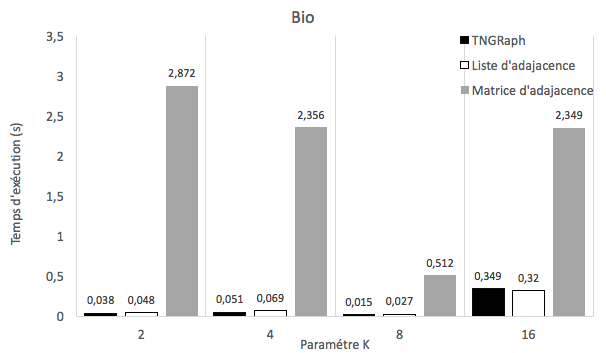
\includegraphics[scale=0.5]{ressources/image/Tests/rep-bio.png}}\hspace{3em}
			%\subfloat[{web-edu. \label{fig:testdom1}}]
			%{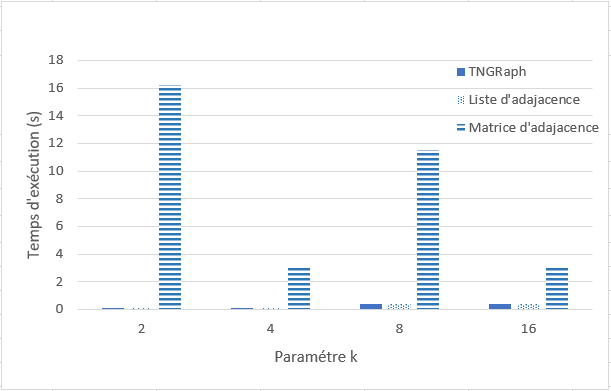
\includegraphics[scale=0.5]{ressources/image/Tests/rep-web-edu.png}}\hspace{3em}
			%\subfloat[{web-polblogs. \label{fig:testdom3}}]
			%{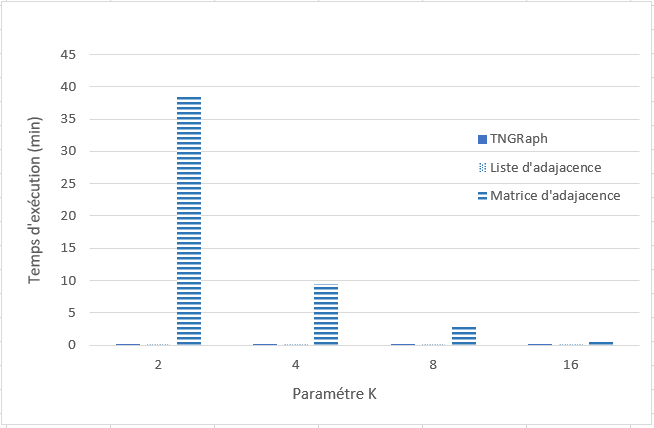
\includegraphics[scale=0.5]{ressources/image/Tests/rep-web-polblogs.png}}\hspace{3em}
			
			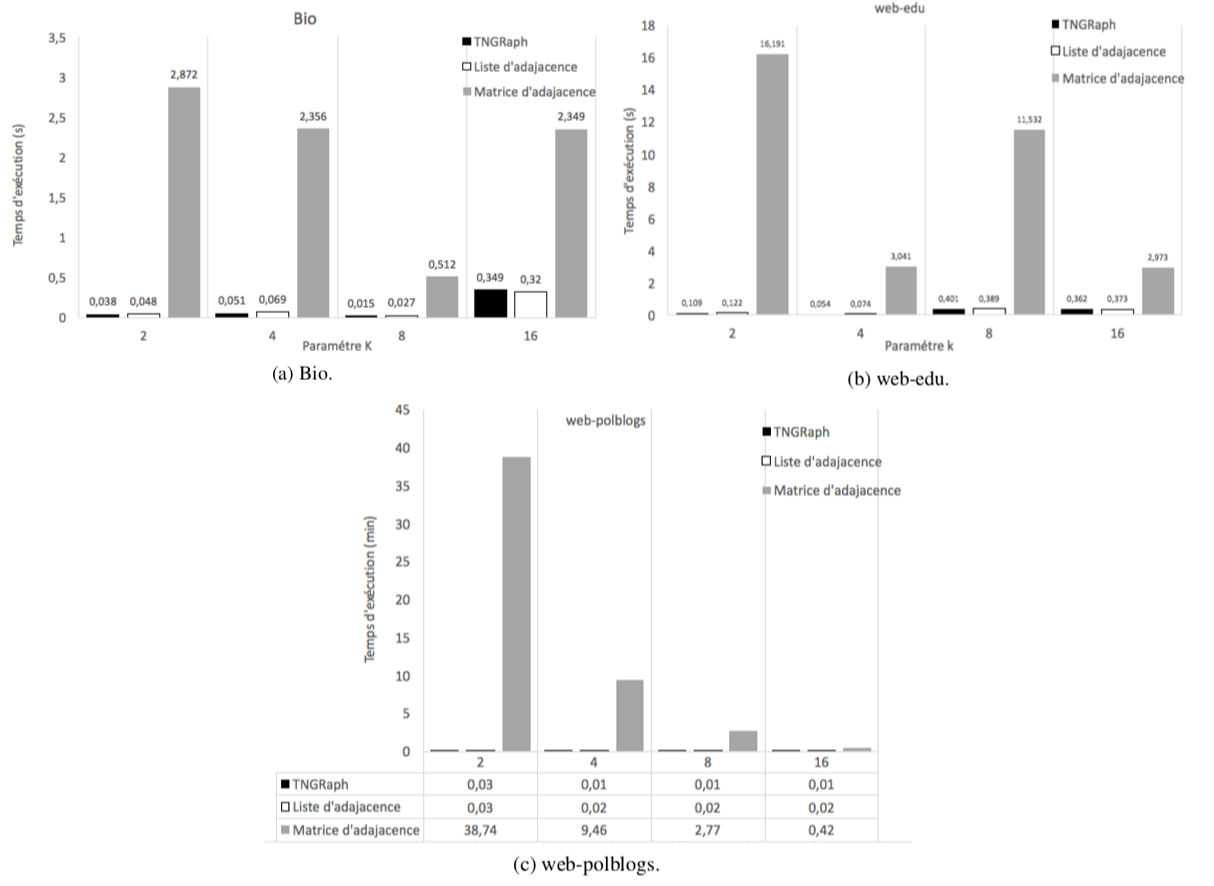
\includegraphics[scale=0.4]{ressources/image/Tests/tst.png}
			\caption{Résultats de tests du moteur $K^2$-Grace selon les différents types de représentations du graphe en entrée.}
			\label{fig:test-rep}
		\end{center}
	\end{figure}
			
Les graphes de la figure  \ref{fig:test-rep} représentent la variation du temps d'exécution de la méthode $k^2$-trees selon les différentes représentations du graphe en entrée appliquée sur trois graphes de tests : Bio, web-edu et web-polblogs. Cette compression a été effectuée avec un ordre initial,et avec différentes valeurs de k. 
Nous constatons d'après les trois figures que l'utilisation des trois représentations donne des temps d'exécution totalement différents. Nous remarquons que si l'écart existant dans le temps d'exécution  entre l'utilisation de la matrice d'adjacence  et les deux autres structures peut être acceptable pour les petits graphes comme bio qui comptent 490 nœuds, il ne peut être toléré pour le cas des grands graphe comme web-edu et web-polblogs.
En effet, nous avons obtenu, dans le cas du graphe bio, un temps d'exécution entre 2 et 3 secondes dans le cas de l'utilisation de la matrice d'adjacence et un temps d'exécution entre 0,015 et 0,4 seconde dans les deux autres cas. Cependant, le cas du graphe web-polblogs donne un temps d'exécution de 38 minutes pour k=2 lorsque le l'arbre est construit en utilisant la matrice d'adjacence et un temps d'exécution de 0,03 secondes dans le cas des deux autres structures. Nous pensons que cela revient au temps que prend la machine pour charger la matrice d'adjacence en mémoire centrale qui devient de plus en plus important lorsque la taille du graphe est grande. De ce fait, nous utiliserons uniquement la structure TNGraph pour la suite des tests.

			\subsection{Analyse de l'impact du paramètre k}
			Les figures \ref{fig:K2-paraK-NBbits} et\ref{fig:K2-paraK-Ratio} représentent respectivement l'évolution du nombre de bits par nœud et du ratio de compression en fonction des différentes valeurs du paramètre K. La compression a été appliquée sur différents graphes de test statiques issus de plusieurs domaines et avec différentes caractéristiques pour avoir une meilleure analyse. Les graphes utilisés dans ce test sont : bio, web-edu, web-polblogs, wiki et soc-Epinions. Cette compression a été effectuée avec un ordre initial et sans aucun pré-traitement.
%, avec comme paramètres :  (a voir aprés avec hafsa les noms des par).
 Nous avons varié le paramètre K entre 2 et 16.
			
\begin{figure}[H]
	\centering
	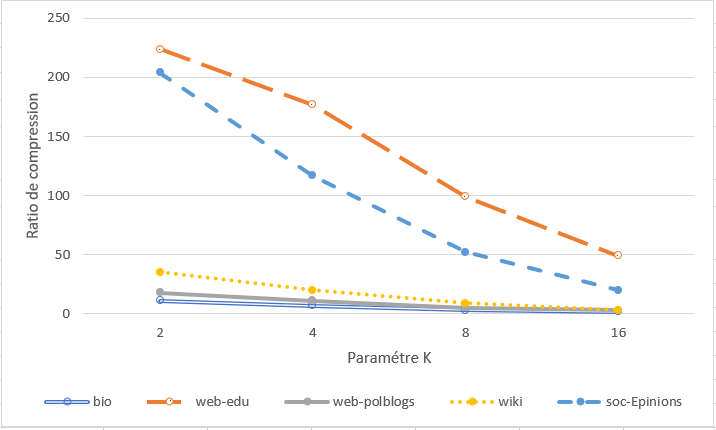
\includegraphics[scale=0.8]{ressources/image/Tests/K2-paraK-Ratio.png}
	
	\caption{Résultats de compression de $K^2$-Grace : Ratio de compression du moteur $K^2$-Grace en fonction du paramètre K (cas statique)}
	\label{fig:K2-paraK-Ratio}
\end{figure}

D'après les résultats obtenues dans la figure \ref{fig:K2-paraK-Ratio}, nous remarquons que le ratio de compression diminue quand k prend des valeurs plus grandes et atteint sa valeur minimale (exemple : 20 pour soc-Epinions) quand K=16. Ainsi, nous constatons que plus le k est petit plus le ratio de compression est optimal. En effet, pour des petites valeurs de K, l'arbre a plus de niveaux, mais il est moins large et le nombre de ses feuilles est plus petit (petites sous matrices finales) ce qui réduit la taille de l'arbre et donne une meilleur qualité de compression. Nous avons pu aussi confirmer cette hypothèse avec le nombre de bits par nœuds obtenu dans les différents cas et qui est représenté dans la figure \ref{fig:K2-paraK-NBbits}. Nous observons que le nombre de bits par nœud augmente de manière exponentielle en fonction du k et atteint sa valeur maximale (exemple 917 938 bits par nœud) quand K est à 16. Le nombre de bits augmente avec les grandes valeurs de k reflétant ainsi une augmentation dans la taille du graphe en sortie.

\begin{figure}[H]
	\centering
	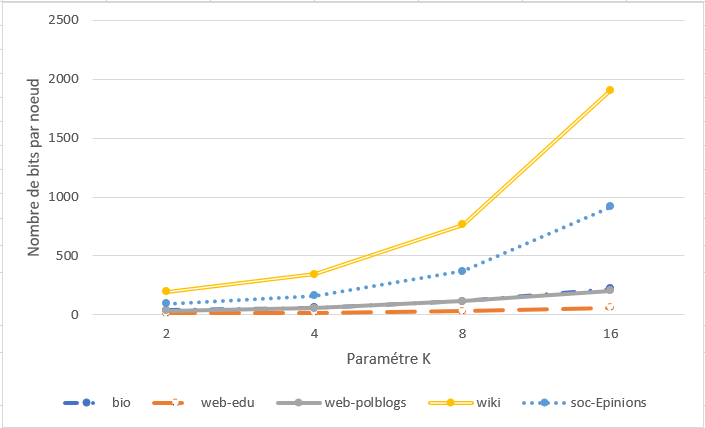
\includegraphics[scale=0.8]{ressources/image/Tests/K2-paraK-NBbits.png}
	
	\caption{Résultats de compression de $K^2$-Grace : Nombre de bits par nœuds en fonction du paramètre K}
	\label{fig:K2-paraK-NBbits}
\end{figure}		


Nous nous sommes aussi intéressées à l'étude de l'effet du paramètre k sur les performances de compression dans le cas des graphes dynamiques. Nous présentons dans la figure \ref{fig:K2-dyn-paraK-NBbits} les résultats obtenus pour ce type de graphe. Les graphes utilisés dans ce test sont : aves-weaver-social, reptilia-tortoise-network-bsv et reptilia-tortoise-network-fi. Ces graphes sont représenté avec leurs captures initiales (sans aucun pré-traitement).


\begin{figure}[H]
	\centering
	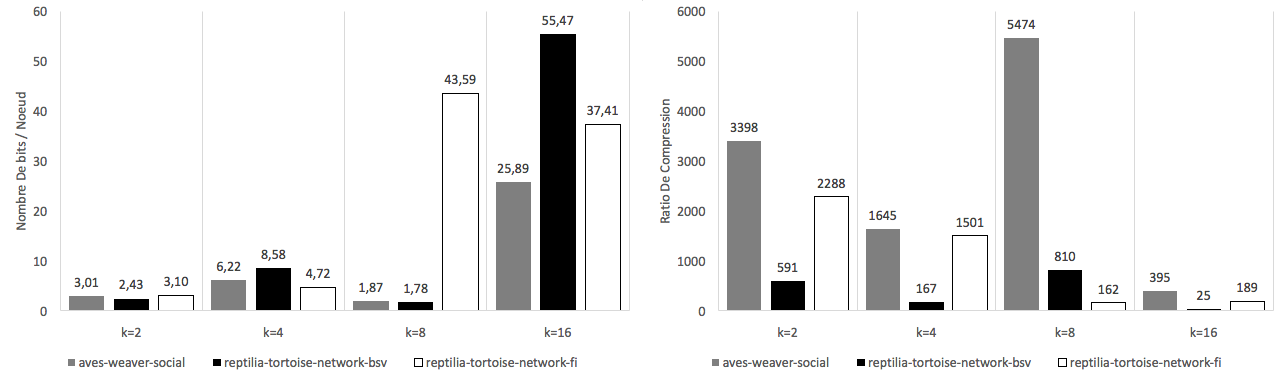
\includegraphics[scale=0.38]{ressources/image/ratioik2.png}
	
	\caption{Résultats de compression de $K^2$-Grace : Nombre de bits par nœuds et Ratio de compression  du moteur en fonction du paramètre K (cas dynamique)}
	\label{fig:K2-dyn-paraK-NBbits}
\end{figure}	
	


A partir de la figure \ref{fig:K2-dyn-paraK-NBbits}, nous remarquons une dégradation des performances dans le cas générales. Cependant, nous obtenons les meilleurs performances pour k=8 dans le cas des deux graphes aves-weaver-social et reptilia-tortoise-network-bsv avec un 1,87 bits par nœud pour le premier graphe et 1,78 bits par nœud pour le deuxième graphe. De ce fait, l'hypothèse que nous avons annoncée dans le cas des graphes statiques ne peut être généraliser dans le cas des graphes dynamiques où nous avons obtenu différentes valeurs optimales de k dans les différents graphes. 

\begin{figure}[H]
	\centering
	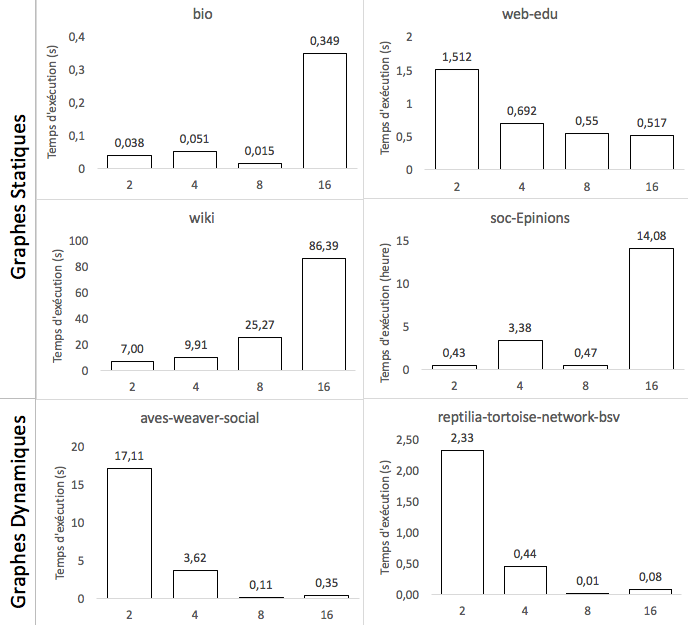
\includegraphics[scale=0.6]{ressources/image/Tests/K2-Texec.png}
	
	\caption{Résultats de compression de $K^2$-Grace : Temps de compression en fonction de K}
	\label{fig:K2-Texec}
\end{figure}

La figure \ref{fig:K2-Texec} représente l'évolution du temps d'exécution en fonction du paramètre K. Dans le cas des graphes statiques, nous notons que le temps de compression varie de manière aléatoire et ne dépend pas de la valeur de K. En effet, dans le cas des graphes bio et soc-Epinions nous obtenons des temps d'exécution qui changent de manière aléatoire. Tant dis que dans le cas du graphe web-edu nous obtenons un temps d'exécution qui diminue en fonction de k contrairement au graphe wiki-Vote dans lequel le temps d'exécution  augmente en fonction du paramètre k. Dans le cas des graphes dynamiques, nous remarquons que le temps d'exécution diminue jusqu'à k=8 où il atteint sa valeur minimale pour k=8 et commence à augmenter à partir de cette valeur.
			
			
 \subsection{Étude de l'apport de la phase de pré-traitement }
 
 Durant cette partie de l'évaluation du moteur $k^2$-GraCE, nous nous focaliserons sur l'étude de l'effet de l'utilisation des techniques du module << pré-traitement >> du moteur $k^2$-GraCE. Nous commencerons par étudier l'effet des différents ordres des nœuds dans le cas des graphes orientés. Nous enchainerons par la mesure du gain apporté par la considération de la partie supérieure uniquement de la matrice d'adjacence dans la construction de l'arbre $k^2$-tree pour le cas des graphes non orientés. Finalement, nous présenterons les tests relatifs à l'utilisation d'une matrice de différence dans le cas des graphes dynamiques.
 			
\subsubsection{Étude de l'effet de l'ordre}

\begin{figure}[H]
	\centering
	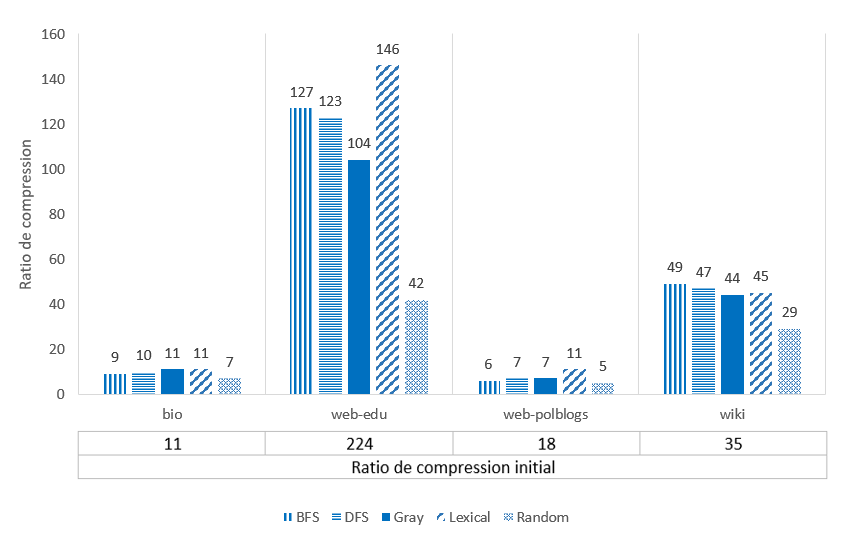
\includegraphics[scale=0.65]{ressources/image/Tests/k2-ordre.png}
	\caption{Résultats de compression de $K^2$-Grace :Ratio de compression selon l'ordre des nœuds}
	\label{fig:K2-ordre }
\end{figure}		

La figure \ref{fig:K2-ordre } représente l'évolution du ratio de compression du moteur $k^2$-Grace sur quatre graphes de compression : bio, web-edu, web-polblogs et wiki. Cette compression a été effectuée en utilisant cinq ordres différents : BFS, DFS, Gray, Lexical et Random avec comme paramètre k=2. Nous remarquons que dans le cas des deux graphes web-edu et web-polblogs qui sont des du web , nous avons obtenu une détérioration des performances de compression pour les différents ordres. Nous justifions cela par le fait que les arbres $k^2$-trees ont été au départ conçus pour exploiter les propriétés de l'ordre initial des nœuds dans la matrice d'adjacence. Cependant, nous remarquons que dans le cas du graphe wiki-Vote, qui est un graphe issu du domaine des réseaux sociaux, nous avons obtenu une amélioration du ratio initial d'un facteur de 1,4 avec les ordres : \gls{dfs}, \gls{bfs}, Gray et Lexical. Pour ce graphe, nous avons obtenu un ratio de compression optimal de 49 pour l'ordre BFS. Dans le cas du graphe bio, nous remarquons que uniquement les ordres Lexical et gray ont permis de garder les même performances que l'ordre initiale. Nous constatons donc que ces ordres donnent de bonnes performances avec les graphes qui ne sont pas issus du domaine du web. En effet, comme nous l'avons déjà noté s'ils ne permettent pas d'améliorer les performances ils ne les détériorent pas.


\subsubsection{Étude de l'effet de l'utilisation de la partie supérieure uniquement de la matrice d'adjacence}


Le tableau \ref{fig:tab-pret } donne les résultats de la compression du moteur $k^2$-Grace appliqué sans et avec pré-traitement sur des graphes non orientés avec un k=2 et un ordre initial des nœuds. Les graphes utilisés sont ca-netscience, Caida et Brightkite. 
 

\begin{figure}[H]
	\centering
	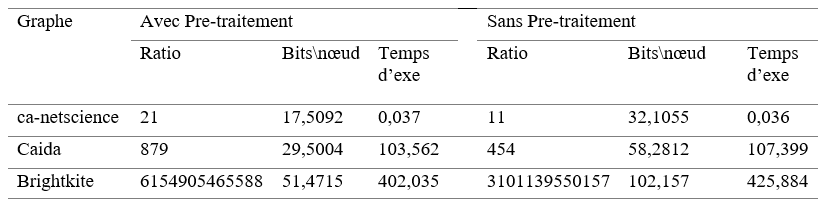
\includegraphics[scale=0.9]{ressources/image/Tests/tab-pret.png}
	\caption{Résultats de compression de $K^2$-Grace avec/sans pré-traitement (cas non orienté)}
	\label{fig:tab-pret }
\end{figure}

Nous observons que le ratio de compression et le nombre de bits par nœud sont nettement meilleurs avec le pré-traitement. Le pré-traitement appliqué sur le graphe non orienté maximise les zones vides dans la matrice d'adjacence en diminuant le nombre de 1 de la moitié ce qui réduit la taille de l'arbre et produit une meilleure qualité de compression. Nous remarquons cela dans le ratio de compression qui double pour les trois graphes. Le temps d'exécution est presque le même entre les deux exécutions car nous construisant la matrice triangulaire supérieure au moment de la lecture directement. Le léger écart noté entre les deux exécutions est du aux comparaisons des indices sources et destinations effectuées pour construire la matrice. 

La figure \ref{fig:gain } présente le gain obtenue après l'application du pré-traitement sur les graphes non orientés, nous remarquons que le gain est aux alentours du double pour tous les graphes. Cela prouve que le pré-traitement améliore clairement la qualité de compression tout en offrant la possibilité d'extraire toutes les informations incluses dans le graphe original.

\begin{figure}[H]
	\centering
	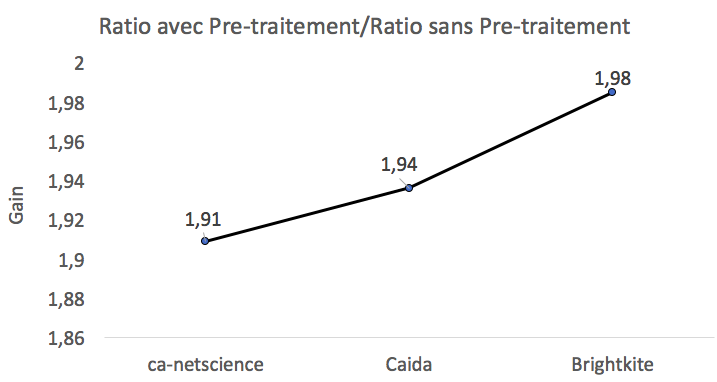
\includegraphics[scale=0.5]{ressources/image/Tests/gain.png}
	
	\caption{Gain de compression de $K^2$-Grace avec le pré-traitement}
	\label{fig:gain }
\end{figure}


\subsubsection{Étude de l'effet de l'utilisation d'une matrice de différence}

Dans cette partie, nous évaluerons l'effet de l'utilisation de la matrice de différence pour la construction de l'arbre sur les performances de compression. Comme les tests précédents ont montré que qu'il n'existe pas de valeur optimale pour le k qui améliore ces derniers, nous effectuerons les tests de cette phase pour différentes valeurs de k. Le tableau de la figure \ref{res-dyn-tst} donne les valeurs des trois (03) métriques considérées en fonction du valeurs de k.


\begin{figure}[H]
	\centering
	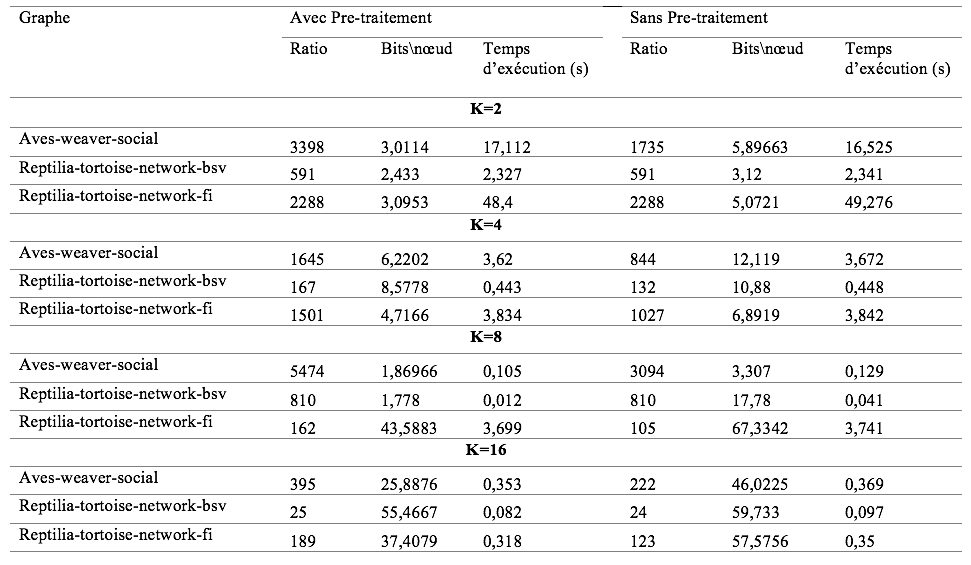
\includegraphics[scale=0.48]{ressources/image/ik2.png}
	\caption{Résultats de compression de $K^2$-Grace avec/sans pré-traitement (cas dynamique)}
	\label{res-dyn-tst}
\end{figure}

Nous remarquons que nous obtenons dans tout les un temps d'exécution presque égale. Le léger écart noté dans le cas de l'utilisation du pré-traitement représente le temps nécessaire pour le calcule de la matrice de différence. 
Pour le graphe aves-weaver-social, nous remarquons que le ratio de compression (resp. le nombre de bits par nœud) diminue (resp. augmente) de moitié (resp. du double) pour toute les valeurs de k. Pour le deuxième graphe reptilia-tortoise-network-bsv, nous observons bien que les performances (ratio et nombre de bits par lien) restent les même dans les deux cas sans et avec pré-traitement. Tant dis que le troisième graphe, nous remarquons que nous obtenons les même performances pour k=2 et que nous perdons en performances quand le k prend des valeurs plus grandes. Pour mieux illustrer ces observation nous fournissons dans la figure \ref{perte } la courbe représentant le rapport entre le ratio de compression avant et après l'utilisation du pré-traitement. 


\begin{figure}[H]
	\centering
	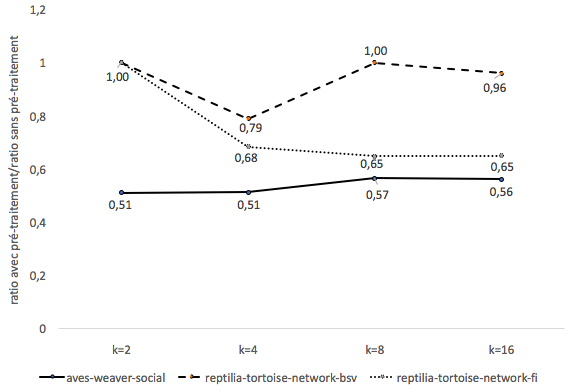
\includegraphics[scale=0.5]{ressources/image/perteIk2.png}
	
	\caption{Ratio de avec pré-traitement/ Ratio de sans pré-traitement}
	\label{perte }
\end{figure}

Nous constatons donc que l'utilisation de ce module n'a pas améliorer les performances de compression dans le cas des trois graphes. Cela est du à la nature leurs captures successives qui ne partagent presque aucun lien en commun engendrant ainsi soit la même matrice initiale ou une matrice de différence plus dense que celle du graphe initial.



	\section{Évaluation du moteur P-GraCE}
	
	Nous évaluerons, dans cette partie, les quartes approches de compression par extraction de motifs incluses dans le moteur P-GraCE. Nous commencerons par l'approche basée sur les propriétés de la matrice d'adjacence où nous allons étudier l'influence du type et de la taille des motifs sur les mesures de performances.  Nous enchainerons par la suite avec l'évaluation des performances de compression par extraction de motifs en utilisant des méthodes de détection de communautés. Nous étudierons aussi le rondement du beam-search en fonction du niveau d'agrégation. Finalement, nous présenterons les différents tests relatifs à la méthode de compression que nous avons proposée: DDSM qui est destinée aux graphes dynamiques.
	
	\subsection{Étude de l'influence du type et de la taille des motifs dans les méthodes basées sur la matrice d'adjacence :}
	
	Durant cette partie, nous présenterons les résultats obtenus lors de l'évaluation de l'extraction de motifs à partir de la matrice d'adjacence. La figure \ref{fig:test-m} illustre l'évolution du ratio de compression en fonction de la taille du motif pour les trois classes de motifs offertes par le moteur P-GracE.
		\begin{figure}[H]
		\begin{center}
		
			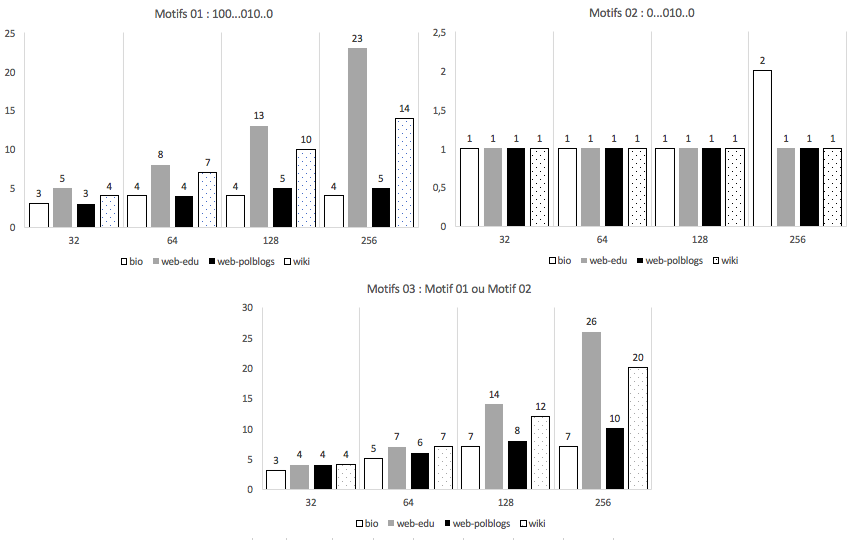
\includegraphics[scale=0.55]{ressources/image/m12.png}
			
			
			
			\caption{Le ratio de compression en fonction de la taille du motif.}
			\label{fig:test-m}
		\end{center}
	\end{figure}
	
	Dans le cas de la première et la troisième classe de motif, nous remarquons une amélioration du ratio de compression lorsque la taille des motifs prend des grandes valeurs. Cette observation est du au gain obtenu en remplaçant des motifs de taille $2^n$ bits par n bits, par exemple les motifs de taille 256bits seront remplacés par uniquement 8bits. Pour la deuxième classe de motif, le ratio de compression est resté presque constant pour différentes valeurs de la taille des motifs. Nous remarquons aussi que ce dernier est égale à 1 dans la majorité des cas signifiant ainsi que le taille du graphe en sortie est égale à la taille du graphe initial. Ce résultat ne peut être obtenu que dans le cas où aucun motif n'a été trouvé dans la matrice d'adjacence. Nous constatons donc que les motifs de cette deuxième classe sont peu fréquents dans les matrices d'adjacence des graphes réels. 
	
	
	
	%\subsection{Évaluation de l'utilisation des méthodes de clustering :}
	
	\subsection{Évaluation de l'algorithme du beam-search :}
	
  Durant cette section, nous considérons le cas des graphes non orientés et étiquetés. Nous évaluerons le rondement de compression de l'algorithme du beam-search sur ces derniers tout en prêtant attention au temps d'exécution. Le tableau ci-dessous résume les résultats obtenus.
  

	\begin{figure}[H]
	
			
			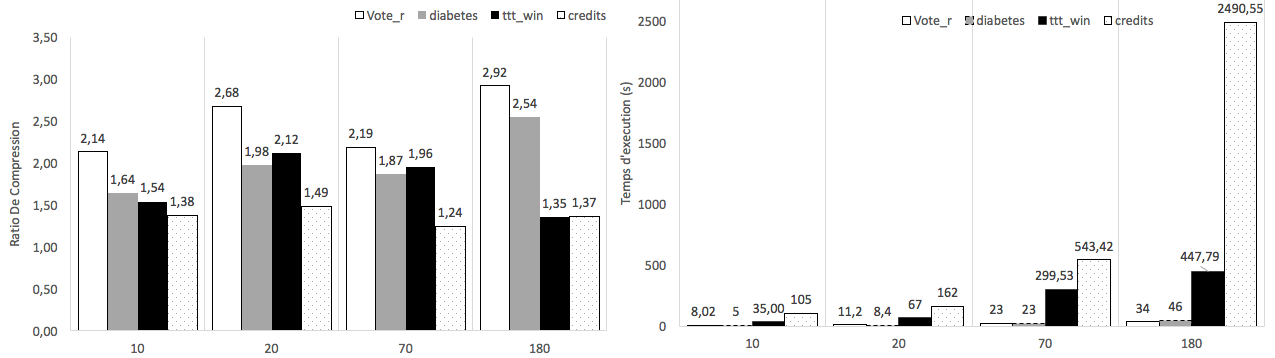
\includegraphics[scale=0.37]{ressources/image/beam.png}
			
			\caption{Résultats des tests du beam-search.}
			\label{fig:test-beam}
	
	\end{figure}
	
	%%% Ajouter le tableau des resulats obtenus 
	
	  La figure \ref{fig:test-beam} illustre les résultats de test obtenus pour différents graphes en fonction du nombre d'itération de l'algorithme (le niveau d'agrégation). Nous constatons une amélioration du ratio de compression dans le majorité des cas. En contre partie, nous remarquons que le temps d'exécution  augmente surtout dans le cas des grands graphes. Le choix du nombre d'itérations (niveau de la hiérarchie d'agrégation) dépend des performances voulues. Cependant, nous pensons qu'un  nombre d'itération égale 70 offre déjà un bon compromis entre le temps d'exécution et le ratio de compression.
	
	
	\subsection{Évaluation de la méthode DDSM :}
	
	Nous présenterons dans cette partie, les tests relatifs à la méthode que nous avons proposée. Nous étudierons les performances obtenues en fonction du nombre de fonctions de hachage utilisées dans le processus de découverte et d'étiquetage des sous-structures. 
\begin{figure}[H]
	
	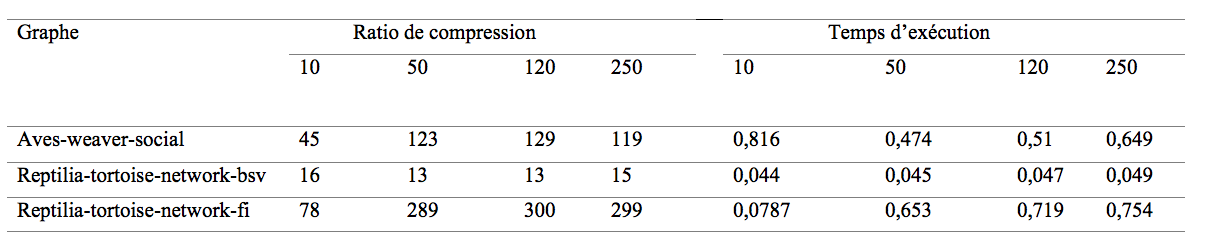
\includegraphics[scale=0.4]{ressources/image/grDDSM.png}
	\label{fig:perte }
	\caption{Résultats de la méthode DDSM}
\end{figure}
		\begin{figure}[H]
		\begin{center}
		 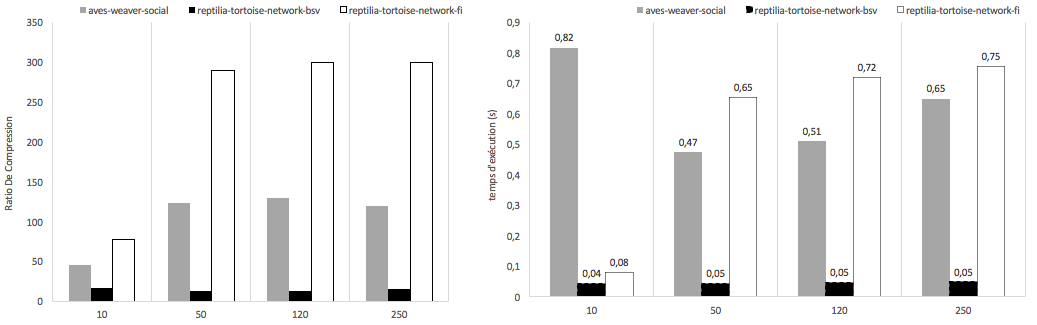
\includegraphics[scale=0.45]{ressources/image/DDSM.png}
			
			
			\caption{Résultats des tests de la méthode DDSM.}
			\label{fig:test-ddsm}
		\end{center}
	\end{figure}
	
	Nous remarquons que la méthode que nous avons proposée offre de très bon résultats par rapport au temps d'exécution qui ne dépasse pas une (01) seconde pour toutes les exécutions. Pour le ratio de compression, nous constatons une amélioration significative qui commence à se stabiliser à partir du moment où le nombre de permutations dépasse 50. 
	
	\begin{figure}[H]
		
		 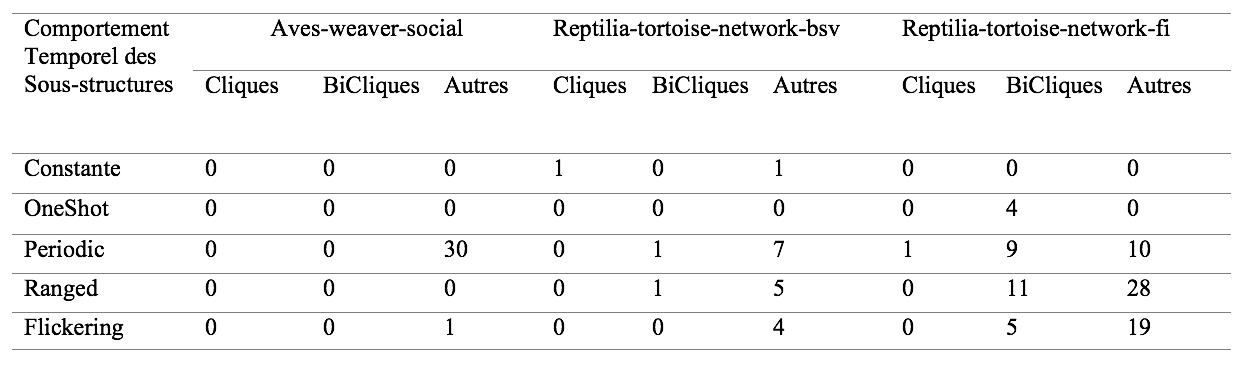
\includegraphics[scale=0.38]{ressources/image/statDDSM.png}
			
			
			\caption{Statistique des différentes types de sous-structures découvertes}
			\label{fig:stat-DDSM}
		
	\end{figure}	
	
	Nous fournissons dans la figure \ref{fig:stat-DDSM} les différentes sous-structures découvertes pour un exemple d'exécution avec 50 permutations. Dans le cas du graphe Aves-weaver-social, nous remarquons que nous obtenons 30 sous-structures denses qui apparaissent de manière périodique et une seule sous-strcuture qui apparait de manière aléatoire. Les sous-structures périodiques représentent donc des utilisateurs du réseaux qui s'envoient des messages  périodiquement (exemple: réunion dans un contexte de télé-travaille, des groupes d'étude, ...). Dans les deux autres réseaux qui font parties des réseaux d'interaction des animaux nous remarquons des sous-structures constantes qui représente peut être des animaux appartenant à un même troupeau. Nous observons aussi des sous-strcutures périodiques qui peuvent être interpréter comme des chasses d'animaux pour avoir de la nourriture. Un autre type sont les sous-structures qui apparaissent dans une seule période représentant en générale le phénomène de couplage chez les animaux dont des périodes bien précises.
	
	DDSM offre ainsi non pas uniquement la compression du graphe initiale mais aussi la possibilité de l'analyser et d'interpréter les informations les plus pertinentes incluses dans ce dernier.
	
	\section{Comparaison entre les différentes méthodes:}
	
	Après avoir évaluer les différentes configuration possibles des deux moteurs : $k^2$-GraCE et P-GraCE, nous nous intéresserons dans cette partie à établir une étude comparative entre les méthodes implémentés dans les deux moteurs ainsi que les classes auxquelles elles appartiennent. Cette partie sera donc organisée en trois sous-section chacune englobant les méthodes de compression acceptant le même type de graphe en entrée.
	
	\subsection{Graphes orientés statiques :}
\begin{figure}[H]
		\begin{center}
		 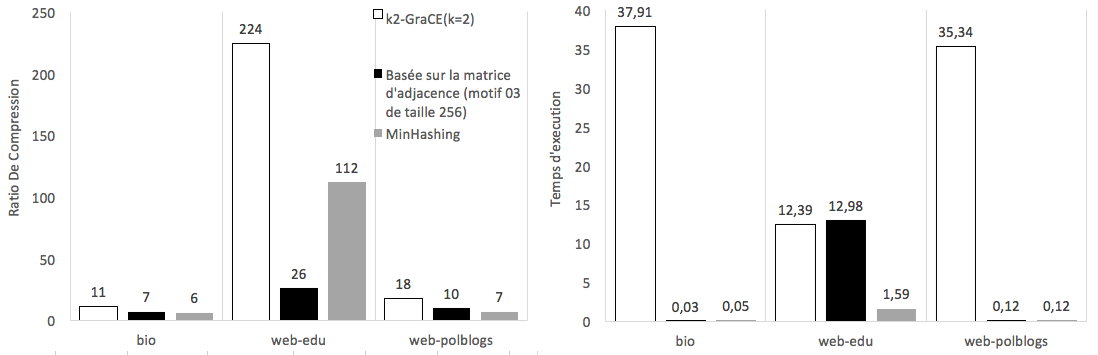
\includegraphics[scale=0.4]{ressources/image/compNon.png}
			
			
			\caption{Comparaison entre les méthodes destinées aux graphes statiques orientés.}
			\label{fig:comp-dyn}
		\end{center}
	\end{figure}	
	
	Nous considérons dans cette partie les graphes orientés: bio, web-edu et web-polblogs, pour comparer entre trois méthodes de compression destinées pour ce type de graphe. Nous utiliserons pour cela deux métriques : le ratio de compression (figure à gauche) et le temps d'exécution (figure à droite). Nous remarquons que le moteur $k^2$-GraCE donne les meilleurs résultats en terme d'espace mémoire (le meilleur ratio). Cependant, il donne le plus grand temps d'exécution. Nous observons aussi que les deux autres méthodes donnent des résultats presque équivalents dans le des graphes bio et web-polblogs, et que la techniques du Minhashing donnent un meilleur résultat dans le cas du graphe web-edu avec un ratio de 112 vs un ratio de 26 pour la méthode basée sur la matrice d'adjacence. 
	
	\subsection{Graphes non orientés statiques :}
	
	\subsection{Graphes dynamiques :}
	
	Dans cette partie, nous allons comparer entre les deux méthodes de compression destinées aux graphes dynamiques qui sont incluses, la première dans le moteur $k^2$-GraCE et la deuxième dans le moteur P-GraCE et qui représente un nouveau schéma de compression que nous proposons. La figure \ref{fig:comp-dyn} montre les résultat des deux méthodes de compression en choisissant les valeurs optimales de leurs paramètres.
	
	\begin{figure}[H]
		\begin{center}
		 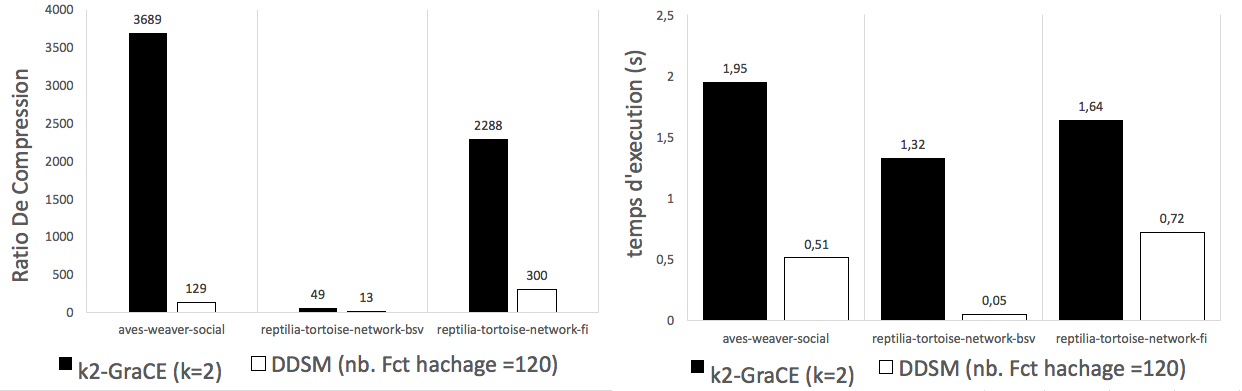
\includegraphics[scale=0.4]{ressources/image/dynComp.png}
			
			
			\caption{Comparaison entre les méthodes destinées aux graphes dynamiques.}
			\label{fig:comp-dyn}
		\end{center}
	\end{figure}
	
	
	Nous remarquons que la ratio de compression est meilleur dans le moteur $k2$-GraCE. En effet, la méthode DDSM donne un ratio de compression très faible en le comparant avec le moteur $k^2$-GraCE (exemple: 3689 vs 129 pour le graphe aves-social-network). Cependant, nous observons bien que le temps d'exécution est nettement meilleur dans le cas de notre méthode. Nous rappelons aussi que notre méthode permet d'extraire les sous-graphes et les communautés les plus denses (les plus importantes) ainsi que leur comportement temporel avec un accès directe alors que le moteur $k^2$-GraCE nécessite un traitement supplémentaire qui peut être lourd dans le cas des grands graphes. 
	
	 
	
	\section{Conclusion}
	
	A travers ce chapitre,  nous avons pu évaluer nos deux moteurs tout en étudiant l'effet de différentes configurations sur leurs performances. Des datasets de domaines hétérogènes ont été employés durant cette étape afin de déduire l'influence de ces derniers sur le choix de l'algorithme de compression. Nous avons opté pour trois métriques d'évaluation : ratio de compression, le nombre de bits par nœuds et le temps d'exécution de l'algorithme de compression.
	
	Dans le cas du moteur $k^2$-GraCE, nous avons constaté que l'utilisation de la matrice d'adjacence pour la construction de l'arbre est trop couteuse en temps d'exécution. L'utilisation de la structure proposée dans la bibliothèque \gls{snap} donne des résultats nettement meilleurs pour cette métrique. Nous avons aussi observé que le choix du paramètre k influence fortement sur les performances de la compression. Selon les résultats obtenus, la valeur optimale dans tout les cas est bien k=2. De plus, nous avons constaté que l'utilisation d'un ré-ordonnancement des nœuds n'est intéressante que dans le cas des graphes autres que les graphes du web où nous avons obtenu une amélioration du ratio de compression d'un facteur de 1,4 dans le cas du graphe wiki-Vote. La généralisation  proposée pour le cas des graphes statiques non orientés permet de doubler le ratio de compression améliorant ainsi la qualité de la compression. D'autre part, nous avons remarqué que l'utilisation du graphe original dans le cas dynamique donne de meilleurs résultats. En effet, nous avons constaté que l'utilisation de la matrice de différence n'est bénéfique que dans le cas où les captures possèdent un degré élevé de ressemblance des liens, ce qui n'est généralement pas le cas dans les graphes réels.
	
	Le deuxième moteur, P-GraCe, permet de compresser le graphe en entrée avec ses sous-structures les plus importantes. Les tests ont montré qu'il n'est pas intéressant d'utiliser le troisième type de motifs dans les méthodes basées sur les propriétés de la matrice d'adjacence car il est peu fréquent dans les graphes réels. Pour le beam-search, nous avons bien remarqué que le niveau d'agrégation doit être choisi d'une manière qui assure un compromis entre le temps d'exécution et le ratio de compression. 
	%% ajouter Condense	
	Finalement, l'évaluation de la méthode que nous proposons a montré qu'elle donne des résultats compétitifs en terme du temps de compression. Certes, le moteur k2-GraCE offre un meilleur ratio dans le cas dynamique mais il n'offre les même avantages que la méthode que nous proposons. En effet, le résultat obtenu par DDSM permet une analyse très rapide des communautés et leurs comportement temporels.
	
	
	%% ajouter conclusion des differentes methdoes
	Nous constatons à travers cette étude que l'utilisation du moteur $k^2$-GraCE est meilleur dans le cas où le but est de diminuer la taille du graphe uniquement. Cependant, le moteur P-GraCE permet d'avoir des informations interprétables qui aident dans l'analyse du graphe car il permet de synthétiser l'information incluse dans le graphe initiale sous forme des sous-structures les plus pertinentes.
	
	
	
	
	
	
	
	
	
	
	
	
	
	
	
	
	
	
	
	
	
	
	
	
	
	
	